%%%%%%%%%%%%%%%%%%%%%%%%%%%%%%%%%%%%%%%%%%%%%%%%%%%%%%%%%%%%%%%%%%%%%%
%%  disstemplate.tex, to be compiled with latex.		     %
%%  08 April 2002	Version 4				     %
%%%%%%%%%%%%%%%%%%%%%%%%%%%%%%%%%%%%%%%%%%%%%%%%%%%%%%%%%%%%%%%%%%%%%%
%%								     %
%%  Writing a Doctoral Dissertation with LaTeX at		     %
%%	the University of Texas at Austin			     %
%%								     %
%%  (Modify this ``template'' for your own dissertation.)	     %
%%								     %
%%%%%%%%%%%%%%%%%%%%%%%%%%%%%%%%%%%%%%%%%%%%%%%%%%%%%%%%%%%%%%%%%%%%%%


\documentclass[12pt]{report}	% The documentclass must be ``report''.

\usepackage{utdiss2}  		% Dissertation package style file.


%%%%%%%%%%%%%%%%%%%%%%%%%%%%%%%%%%%%%%%%%%%%%%%%%%%%%%%%%%%%%%%%%%%%%%
% Optional packages used for this sample dissertation. If you don't  %
% need a capability in your dissertation, feel free to comment out   %
% the package usage command.					     %
%%%%%%%%%%%%%%%%%%%%%%%%%%%%%%%%%%%%%%%%%%%%%%%%%%%%%%%%%%%%%%%%%%%%%%

\usepackage{amsmath,amsthm,amsfonts,amscd} 
				% Some packages to write mathematics.
\usepackage{eucal} 	 	% Euler fonts
\usepackage{verbatim}      	% Allows quoting source with commands.
\usepackage{makeidx}       	% Package to make an index.
\usepackage{psfig}         	% Allows inclusion of eps files.
\usepackage{epsfig}         	% Allows inclusion of eps files.
\usepackage{citesort}         	% 
\usepackage{url}		% Allows good typesetting of web URLs.
\usepackage{ctable}
\usepackage{float}
%\usepackage{draftcopy}		% Uncomment this line to have the
				% word, "DRAFT," as a background
				% "watermark" on all of the pages of
				% of your draft versions. When ready
				% to generate your final copy, re-comment
				% it out with a percent sign to remove
				% the word draft before you re-run
				% Makediss for the last time.

\pdfpageattr {/Group << /S /Transparency /I true /CS /DeviceRGB>>}

\author{Benjamin Mark Cochran}  	% Required

\address{ben.cochran@utexas.edu}  % Required

\title{A Framework for Spatio-Temporal Querying Amongst Mobile
Devices}
                                                    % Required

%%%%%%%%%%%%%%%%%%%%%%%%%%%%%%%%%%%%%%%%%%%%%%%%%%%%%%%%%%%%%%%%%%%%%%
% NOTICE: The total number of supervisors and other members %%%%%%%%%%
%%%%%%%%%%%%%%% MUST be seven (7) or less! If you put in more, %%%%%%%
%%%%%%%%%%%%%%% they are put on the page after the Committee %%%%%%%%%
%%%%%%%%%%%%%%% Certification of Approved Version page. %%%%%%%%%%%%%%
%%%%%%%%%%%%%%%%%%%%%%%%%%%%%%%%%%%%%%%%%%%%%%%%%%%%%%%%%%%%%%%%%%%%%%

%%%%%%%%%%%%%%%%%%%%%%%%%%%%%%%%%%%%%%%%%%%%%%%%%%%%%%%%%%%%%%%%%%%%%%
%
% Enter names of the supervisor and co-supervisor(s), if any,
% of your dissertation committee. Put one name per line with
% the name in square brackets. The name on the last line, however,
% must be in curly braces.
%
% If you have only one supervisor, the entry below will read:
%
%	\supervisor
%		{Supervisor's Name}
%
% NOTE: Maximum three supervisors. Minimum one supervisor.
% NOTE: The Office of Graduate Studies will accept only two supervisors!
% 
%
\supervisor
	{Christine Julien}

%%%%%%%%%%%%%%%%%%%%%%%%%%%%%%%%%%%%%%%%%%%%%%%%%%%%%%%%%%%%%%%%%%%%%%
%
% Enter names of the other (non-supervisor) members(s) of your
% dissertation committee. Put one name per line with the name
% in square brackets. The name on the last line, however, must
% be in curly braces.
%
% NOTE: Maximum six other members. Minimum zero other members.
% NOTE: The Office of Graduate Studies may restrict you to a total
%	of six committee members.
%
%
\committeemembers
	{William Bard}

%%%%%%%%%%%%%%%%%%%%%%%%%%%%%%%%%%%%%%%%%%%%%%%%%%%%%%%%%%%%%%%%%%%%%%

\previousdegrees{B.S.C.E.}
     % The abbreviated form of your previous degree(s).
     % E.g., \previousdegrees{B.S., MBA}.
     %
     % The default value is `B.S., M.S.'

%\graduationmonth{...}      
     % Graduation month, either May, August, or December, in the form
     % as `\graduationmonth{May}'. Do not abbreviate.
     %
     % The default value (either May, August, or December) is guessed
     % according to the time of running LaTeX.

%\graduationyear{...}   
     % Graduation year, in the form as `\graduationyear{2001}'.
     % Use a 4 digit (not a 2 digit) number.
     %
     % The default value is guessed according to the time of 
     % running LaTeX.

%\typist{...}       
     % The name(s) of typist(s), put `the author' if you do it yourself.
     % E.g., `\typist{Maryann Hersey and the author}'.
     %
     % The default value is `the author'.


%%%%%%%%%%%%%%%%%%%%%%%%%%%%%%%%%%%%%%%%%%%%%%%%%%%%%%%%%%%%%%%%%%%%%%
% Commands for master's theses and reports.			     %
%%%%%%%%%%%%%%%%%%%%%%%%%%%%%%%%%%%%%%%%%%%%%%%%%%%%%%%%%%%%%%%%%%%%%%
%
% If the degree you're seeking is NOT Doctor of Philosophy, uncomment
% (remove the % in front of) the following two command lines (the ones
% that have the \ as their second character).
%
\degree{Master of Science in Engineering}
\degreeabbr{M.S.E.}

% Uncomment the line below that corresponds to the type of master's
% document you are writing.
%
\masterreport
%\masterthesis


%%%%%%%%%%%%%%%%%%%%%%%%%%%%%%%%%%%%%%%%%%%%%%%%%%%%%%%%%%%%%%%%%%%%%%
% Some optional commands to change the document's defaults.	     %
%%%%%%%%%%%%%%%%%%%%%%%%%%%%%%%%%%%%%%%%%%%%%%%%%%%%%%%%%%%%%%%%%%%%%%
%
%\singlespacing
%\oneandonehalfspacing

%\singlespacequote
\oneandonehalfspacequote

\topmargin 0.125in	
        % Adjust this value if the PostScript file output
		% of your dissertation has incorrect top and 
		% bottom margins. Print a copy of at least one
		% full page of your dissertation (not the first
		% page of a chapter) and measure the top and
		% bottom margins with a ruler. You must have
		% a top margin of 1.5" and a bottom margin of
		% at least 1.25". The page numbers must be at
		% least 1.00" from the bottom of the page.
		% If the margins are not correct, adjust this
		% value accordingly and re-compile and print again.
		%
		% The default value is 0.125"

		% If you want to adjust other margins, they are in the
		% utdiss2-nn.sty file near the top. If you are using
		% the shell script Makediss on a Unix/Linux system, make
		% your changes in the utdiss2-nn.sty file instead of
		% utdiss2.sty because Makediss will overwrite any changes
		% made to utdiss2.sty.

%%%%%%%%%%%%%%%%%%%%%%%%%%%%%%%%%%%%%%%%%%%%%%%%%%%%%%%%%%%%%%%%%%%%%%
% Some optional commands to be tested.				     %
%%%%%%%%%%%%%%%%%%%%%%%%%%%%%%%%%%%%%%%%%%%%%%%%%%%%%%%%%%%%%%%%%%%%%%

% If there are 10 or more sections, 10 or more subsections for a section,
% etc., you need to make an adjustment to the Table of Contents with the
% command \longtocentry.
%
%\longtocentry 

%%%%%%%%%%%%%%%%%%%%%%%%%%%%%%%%%%%%%%%%%%%%%%%%%%%%%%%%%%%%%%%%%%%%%%
% Don't put Chapter X: Blah			     %
%%%%%%%%%%%%%%%%%%%%%%%%%%%%%%%%%%%%%%%%%%%%%%%%%%%%%%%%%%%%%%%%%%%%%%

\renewcommand{\chaptername}{}

%%%%%%%%%%%%%%%%%%%%%%%%%%%%%%%%%%%%%%%%%%%%%%%%%%%%%%%%%%%%%%%%%%%%%%
%	Some math support.					     %
%%%%%%%%%%%%%%%%%%%%%%%%%%%%%%%%%%%%%%%%%%%%%%%%%%%%%%%%%%%%%%%%%%%%%%
%
%	Theorem environments (these need the amsthm package)
%
%% \theoremstyle{plain} %% This is the default

\newtheorem{thm}{Theorem}[section]
\newtheorem{cor}[thm]{Corollary}
\newtheorem{lem}[thm]{Lemma}
\newtheorem{prop}[thm]{Proposition}
\newtheorem{ax}{Axiom}

\theoremstyle{definition}
\newtheorem{defn}{Definition}[section]

\theoremstyle{remark}
\newtheorem{rem}{Remark}[section]
\newtheorem*{notation}{Notation}

%\numberwithin{equation}{section}


%%%%%%%%%%%%%%%%%%%%%%%%%%%%%%%%%%%%%%%%%%%%%%%%%%%%%%%%%%%%%%%%%%%%%%
%	Macros.							     %
%%%%%%%%%%%%%%%%%%%%%%%%%%%%%%%%%%%%%%%%%%%%%%%%%%%%%%%%%%%%%%%%%%%%%%
%
%	Here some macros that are needed in this document:


\newcommand{\latexe}{{\LaTeX\kern.125em2%
                      \lower.5ex\hbox{$\varepsilon$}}}

\newcommand{\amslatex}{\AmS-\LaTeX{}}

\chardef\bslash=`\\	% \bslash makes a backslash (in tt fonts)
			%	p. 424, TeXbook

\newcommand{\cn}[1]{\texttt{\bslash #1}}

\makeatletter		% Starts section where @ is considered a letter
			% and thus may be used in commands.
\def\square{\RIfM@\bgroup\else$\bgroup\aftergroup$\fi
  \vcenter{\hrule\hbox{\vrule\@height.6em\kern.6em\vrule}%
                                              \hrule}\egroup}
\makeatother		% Ends sections where @ is considered a letter.
			% Now @ cannot be used in commands.

\makeindex    % Make the index

%%%%%%%%%%%%%%%%%%%%%%%%%%%%%%%%%%%%%%%%%%%%%%%%%%%%%%%%%%%%%%%%%%%%%%
%		The document starts here.			     %
%%%%%%%%%%%%%%%%%%%%%%%%%%%%%%%%%%%%%%%%%%%%%%%%%%%%%%%%%%%%%%%%%%%%%%

\begin{document}

\copyrightpage          % Produces the copyright page.


%
% NOTE: In a doctoral dissertation, the Committee Certification page
%		(with signatures) is BEFORE the Title page.
%	In a masters thesis or report, the Signature page
%		(with signatures) is AFTER the Title page.
%
%	If you are writing a masters thesis or report, you MUST REVERSE
%	the order of the \commcertpage and \titlepage commands below.
%

\begin{center}
The Report committee for Benjamin Mark Cochran \linebreak
Certifies that this is the approved version of the following report:
\end{center}

\commcertpage           % Produces the Committee Certification
						%   of Approved Version page (doctoral)
						%   or Signature page (masters).
						%		20 Mar 2002	cwm
						
\titlepage              % Produces the title page.

%%%%%%%%%%%%%%%%%%%%%%%%%%%%%%%%%%%%%%%%%%%%%%%%%%%%%%%%%%%%%%%%%%%%%%
% Dedication and/or epigraph are optional, but must occur here.      %
%%%%%%%%%%%%%%%%%%%%%%%%%%%%%%%%%%%%%%%%%%%%%%%%%%%%%%%%%%%%%%%%%%%%%%
%
\begin{dedication}
\index{Dedication@\emph{Dedication}}%
For Ashley

$\sqrt{cosx}*cos300x+\sqrt{\left|{x}\right|-0.7}*(4-{x}^{2}{)}^{0.01}$
\end{dedication}


\begin{acknowledgments}		% Optional
\index{Acknowledgments@\emph{Acknowledgments}}%
I would like to send my appreciation and gratitude towards the
University of Texas faculty and staff who have made my adventure in
graduate studies an enriching experience. In the time I have spent
working towards my degree I have undertaken numerous challenges and
projects that I normally would not be able to bring to completion. I
especially would like to thank a few distinguished individuals starting
with Professor Christine Julien for a rewarding exploration of Mobile
Computing topics and for advising me on this project. Second, I'd like
to thank Professor William Bard for the Advanced Embedded Systems course
which was hands down my favorite course and also for serving on my
report committee. Finally, I would like to thank Professor Joydeep Ghosh
for adding some Data Mining techniques and tools to my tool belt for use
in our heavily data-centric world.
\end{acknowledgments}


% The abstract is required. Note the use of ``utabstract'' instead of
% ``abstract''! This was necessary to fix a page numbering problem.
% The abstract heading is generated automatically.
% Do NOT use \begin{abstract} ... \end{abstract}.
%
\utabstract
\index{Abstract}%
\indent
With mobile web browsers holding around eight percent of the global
browser market share in terms of usage, web development for these
platforms is becoming critically important as usage moves from the
desktop towards mobile devices. Recent advances in client side browser
technology like HTML5 and WebSockets have allowed web browser
applications to approach feature parity with thick client desktop
applications. This paper explores the possibility of a real-time online
multiplayer game playable from just a mobile device's web browser. It
does not focus on gameplay or graphics, rather it focuses on the backend
infrastructure needed to support such a game. The framework devised to
support this sort of interaction, Marionette, is well suited towards
addressing sharing of location-specific, short-lived information between
people using their smartphones without the use of any external software
or proprietary software packages on the client side.



\tableofcontents   % Table of Contents will be automatically
                   % generated and placed here.

\listoftables      % List of Tables and List of Figures will be placed
\listoffigures     % here, if applicable.

%%%%%%%%%%%%%%%%%%%%%%%%%%%%%%%%%%%%%%%%%%%%%%%%%%%%%%%%%%%%%%%%%%%%%%
% Actual text starts here.					     %
%%%%%%%%%%%%%%%%%%%%%%%%%%%%%%%%%%%%%%%%%%%%%%%%%%%%%%%%%%%%%%%%%%%%%%
%
% Including external files for each chapter makes this document simpler,
% makes each chapter simpler, and allows for generating test documents
% with as few as zero chapters (by commenting out the include statements).
% This allows quicker processing by the Makediss command file in case you
% are not working on a specific, long and slow to compile chapter. You
% can even change the chapter order by merely interchanging the order
% of the include statements (something I found helpful in my own
% dissertation).
%

\chapter{Introduction}

This paper presents a framework called Marionette for the storage and
querying of spatio-temporal events within the mobile computing domain.
It leverages technology available in mobile browsers today, allowing
them to serve as location aware clients that can execute queries and
create events relative to a particular mobile device's current position. The events are
stored and queried within a network consisting of mobile device web
browsers that are responsible for handling queries within a certain
geographical area referred to as a zone. Bridging the gap between all
the web based clients is a reliable soft real-time communications
backbone called Juggernaut \cite{juggernaut}. Juggernaut uses a channel-based pub-sub
model that allows flexible levels of broadcast communication and even
unicast communication to one subscriber.

Most mobile network enabled games on the market today have to be
implemented at least twice, once for iOS and once for Android. Other
developers opt to support one platform or the other due to the
differences of the respective platforms. Additionally, there are several
other mobile platforms that games could be implemented in but frequently are
skipped over in favor of a mobile OS with more market penetration. Most
of the major players in the mobile browser space use WebKit
\footnote{The WebKit Open Source Project - \url{http://www.webkit.org/}} based
implementations for their web browser, even those used in Blackberry and
Symbian OS devices. The mobile browser space is becoming more attractive
for game developers as well. The \texttt{<canvas>} element in 
HTML5\footnote{HTML5 Standard - \url{http://html5.org/}} along with
support for Scalable Vector Graphics (SVG) within WebKit supported
browsers allows for graphics rendering capability previously unseen without
proprietary plugins such as Adobe Flash Player. It is possible today to
make a simple two dimensional game in a mobile web browser and have the
experience comparable to a two dimensional game written in the device's native
OS thus making them acceptable candidates for mobile game development. 
This paper does not focus on graphics in lieu of what it would take to 
effectively communicate between these client mobile web browsers in 
spatio-temporal contexts.

Marionette aims to enable distributed spatio-temporal information
exchange via something as simple as opening a tab on a web browser 
on a mobile device. Web browsers in general have
historically been limited in their capability for persistent data 
storage\footnote{Prior to WebSQL, web developers were constrained by 
HTTP cookies that had a maximum storage capacity of only 4 Kilobytes} 
and processing\footnote{Javascript engines have improved through optimization, as well as 
libraries and best practices for the Javascript language on the web} 
but are catching up to deliver rich interactive experiences
that rival thick client applications. Most mobile device browsers have
increased storage and access to increased processing power, which is 
advantageous for Marionette because it has virtually no installation 
requirements and can be run on stock mobile browsers. It operates under the hood
within a browser session and presents the potential for not only content
delivery via a web portal, but also for the absorption of spatially 
contextual information based on the user's location and activities.

Besides mobile gaming, Marionette has other potential uses. Picture a
high profile public event such as Austin City Limits (ACL) or South by
Southwest (SXSW), where event participants have a large thirst for
knowledge. These example events are musical in nature and have a lineup
with events happening at various times. The acts are relatively short,
but there are many happening concurrently. Event goers tend to migrate
towards better live performances discovered on-the-fly through word of mouth,
primarily through social networks like Twitter. With Marionette one
could provide a web portal specifically for attendees to create and distribute 
information in a grassroots
fashion where they can get the latest updates and inform other attendees
if there is an act near them that is exceeding expectations and should
not be missed. An application using Marionette can provide static content 
similar to what a typical website would provide such as a
schedule and maps to draw attendees to participate.  While visiting, the 
application can allow users to rate the experiences all around them which 
gets mixed into the static data dynamically in an asynchronous fashion. 
All of the dynamic data has an expiration date, which makes it
short lived and meaningful only for a short period of time which is ideal 
for event attendees as they would not be interested in stale data about 
something that has already happened. The data is
only available to those viewing the service and not shared publicly on a
social network.

This paper also presents a mobile multiplayer online web game entitled
Space Battle! which is built on top of Marionette to allow the game to be played amongst 
mobile browsers. The proposed method for information creation and retrieval 
presented in the next section works well towards determining the location of other 
players within the game. 
A mobile device's physical location determines where it is located inside 
the game, and a player can interact with other players
that are physically nearby. To accomplish these gameplay
goals, Marionette is used as a medium for propagating in game events.

\chapter{Related Work}

\section{Cornerstone Work}

Marionette is based on the work presented in
\cite{zio2011p2p} and
\cite{yoneki2007socio}. In
\cite{zio2011p2p} the authors create a Peer-to-Peer
(P2P) network for the storage and query of short lived events with
spatial context. The authors create a Voronoi tessellation based
segmentation relative to the spatial locations of the nodes in its P2P
overlay network. Marionette uses a similar construct with regards to the
creation of zones which, are created based on other mobile devices nearby, as well
as adopting the same ``range query'' model. When resolving a range query,
Marionette calculates a subset of zones where the circular query area with 
query radius \textit{r} intersects and broadcasts the request to them. If a client 
node matches the query based on locality and object type requested,
it sends the event(s) that matched to the node that originated the
query. The pattern of resolving queries is similar to how it is
performed in \cite{zio2011p2p}. Where Marionette
differs is in the use of a centralized (but scalable) message broker
that keeps tabs on the state of each node in the network as opposed to
being purely P2P. Another difference is that the mobile browsers
themselves can become peers without requiring proxy peers.
One disadvantage with Marionette's methodology is that there is a
dependency on the message broker in favor of true P2P. The flow of
events and then querying for them in \cite{zio2011p2p}
is important towards realizing spatio-temporal information exchange
amongst users that share physical locality.

In \cite{yoneki2007socio}, the authors create a
Socio-Aware Overlay for Publish/Subscribe based communications for Delay
Tolerant Networks (DTNs). It utilizes a concept known as ``Node
Centrality'' to determine communities and broker nodes, those with the
shortest path to all of the other nodes. The zones in Marionette (known
as communities in \cite{yoneki2007socio}) are defined
by the Voronoi tessellation as defined in
\cite{zio2011p2p}, but the concept of using pub-sub to
facilitate communication is prevalent in Marionette. In Marionette, mobile
clients can publish information as well as be subscribers in a few
different levels of spatially progressive granularity ranging from global 
subscriptions to subscriptions where only one client is subscribed. Distributing the
events and queries within zones using a pub-sub methodology allows for
more flexibility architecturally where other
P2P based approaches have to choose their routing protocols carefully
and tie it specifically to a usage model. Flexibility and
scalability are important towards utilizing Marionette for grassroots
deployments and online web gaming as described in the introduction.

In \cite{wang2005event}, the authors define a
spatio-temporal phenomenon as a collection of processes, entities, and
events. Processes bind entities and events, and events cause changes in the
system. A similar concept is presented in
\cite{chen1998event}. In Marionette, events are linked to game entities as every event
has an entity identifier.  Game participants can then query for those events
and use the results to discover how the system has changed over time.

\section{Other Work}

Other related work in the spatio-temporal area includes PeopleNet
\cite{motani2005peoplenet}, where topic specific
`bazaars' are created with the intent of answering topic specific
queries. As \cite{zio2011p2p} mentions, this approach
does not preserve locality in storage. The only commonality that
Marionette has with the bazaar concept is locality in querying. FLORA
\cite{kokku2008enabling} is similar in the sense that
it uses a hybrid P2P and pub-sub architecture, but Marionette spreads the
data throughout the client devices and only utilizes the message broker to
pass messages. Additionally, Marionette does not focus on
networking at the carrier level like FLORA does. It is assumed that the
query propagation bandwidth in this work will be inconsequential next to
audio and visual streaming allowed by most carriers today.

Gander \cite{michel2011gander} is a personalized search
engine for discovering the ``ground truth'' i.e., short lived information
with a spatio-temporal context. The authors insert a relevance component
into their spatio-temporal data model which aims to rank the search
results based on what the user is looking for. Gander shares a similar
end goal with Marionette but their architecture is distributed and does
not utilize a central message broker. GeoRel
\cite{reichenbacher2009geo} is an extension on
traditional location based information systems where spatial, temporal,
and motivational considerations are mixed in. GeoRel mainly focuses on
assigning relevance of static entities to mobile devices. Marionette
differs because there are no static entities; all of the information
contained within the system is dynamic.

WebPark \cite{mountain2007geo} introduces post-query
filters to traditional Global Information Retrieval (GIR) systems adding
additional geographical context. The most interesting post-query filter
added the notion of speed-heading to query results. Based on a mobile device's
current speed and heading, a user could retrieve results along his future
path. Marionette does not currently implement some of the extended
querying capabilities presented in WebPark, opting for multiple
successive range queries as the user's location changes over time
instead. In Secondo \cite{teixeira2006querying}, the
authors create a data model and query language for information retrieval
of moving objects in time and space. The work focuses on extending more
traditional Database Management Systems (DBMS), which implies that the
data be centrally located. With Marionette, the data is distributed
amongst its client nodes, which are moving themselves and queried at
successive time intervals.

\chapter{Technology}

\begin{figure}[h!]
\centering
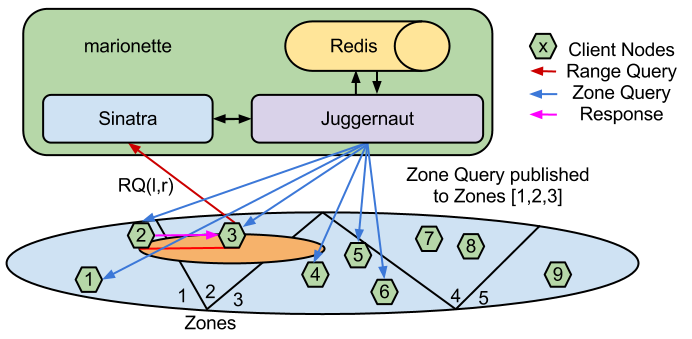
\includegraphics[scale=0.6]{0.png}
\caption{Marionette High Level Architecture}
\label{hla}
\end{figure}

\section{Architecture}

Marionette consists of a pub-sub service provided by Juggernaut backed
by a Redis\footnote{Redis open source, advanced key-value store - \url{http://redis.io/}} 
data store, and a lightweight web application framework
called Sinatra\footnote{Lightweight web applications with Sinatra - \url{http://www.sinatrarb.com/}}. 
Together they allow soft real-time communication between
the mobile devices that are playing the Space Battle! game. Figure
\ref{hla} shows the High Level Architecture (HLA) of
Marionette. It also outlines the concept of zones, which are polygons in
the Voronoi tessellation, and clients distributed within them. Node three
makes a range query with radius r and its current location l and
executes a POST operation to the web server. The server calculates the
zones that overlap the space defined by the range query in orange and
publishes the query to them. The clients in the three zones are notified
of the query and if any client has an event that matches the query, it
gets sent back to node three. If there are multiple matches from
different nodes, node three will also receive them. It is expected 
(but not ensured in the current implementation) that
the node that generated the range query will receive the responses
asynchronously within a set time window and can then act on any
responses received at the end of that time interval.

\section{Server Side}

\subsection{Juggernaut}

Juggernaut is a pub-sub based communications mechanism based on Node.js which provides a
soft real-time connection to clients. It is built on top of Node.js and
is geared towards communication with client web browsers. It supports a
myriad of different browser networking protocols through the use of
Socket.IO, most notably WebSocket and Adobe Flash Socket. Socket.IO is
an extension of WebSocket that adds support for heartbeats, timeouts,
and disconnection support for use in soft real-time web applications
like Marionette. If the client browser does not support WebSockets, it
will fall back to a networking protocol that is supported like Adobe Flash 
Socket with no impact on Juggernaut's functionality. Clients can
subscribe to multiple channels at once, each one having its own callback
on the client side.

\subsection{Node.js}

Node.js\footnote{Node.js, a platform built for easily building fast, 
scalable network applications \linebreak \url{http://nodejs.org/}} is an event 
driven software system that is built from the
ground up to have asynchronous I/O. This allows Node.js applications,
which are mainly server based like Juggernaut, to be highly scalable while minimizing
overhead with non-blocking I/O. Node.js excels at simple POST and GET
processing and is ideal for the communications backbone of this
framework. Additionally, Node.js can span multiple cores and even
multiple machines providing simple scalability.

\subsection{Redis}

Redis is a networked lightweight in-memory key-value data store. The
whole dataset is stored in RAM, but Redis can optionally be configured
for persistence, fulfilling durability requirements. Redis also supports
master-slave replication, which allows Redis to become decentralized. 
Durability and replication are not used within Marionette. A
unique aspect of Redis is that the values it stores can be more than
just strings unlike LevelDB\footnote{LevelDB, A fast and lightweight key/value 
database library by Google. \linebreak \url{http://code.google.com/p/leveldb/}}. 
It can store data types such as lists of strings, sets of
strings, sorted sets of strings, and hashes. There are commands that are
available to each data type. For instance, you can perform operations
like difference, union and intersection on lists, sets and sorted sets.
Every Juggernaut instance uses Redis as its primary data storage mechanism such that it
can provide channel/subscriber data quickly to Node.js connections.

\subsection{Sinatra}

Sinatra is a lightweight web application framework that abstracts
server-side web development in a clean Domain Specific Language (DSL).
It is widely regarded as a barebones Ruby on Rails (RoR).
Sinatra is used to create simple web applications quickly without a lot of configuration.
Several HTML templating options are available for use with Sinatra
making it easy to create simple data and event driven websites. In this
project, asynchronous POST requests from the client web browser are
processed by Sinatra as well as generating the data and event driven
HTML that is displayed.

\section{Client Side}

\subsection{JavaScript}

JavaScript is a dynamically typed scripting language found in any web
browser created since 1996, when it was included in Netscape Navigator
2.0 and Internet Explorer 3.0. The language has been internationally
standardized under the name EMCAScript since 1997. The usage of
JavaScript on client-side web browsers has allowed the creation of
many of the interactive web applications we enjoy today such as Gmail.
Gmail was one of the first web applications to feature an extensive use
of JavaScript, which dispatches user interface events and information
queries back to the web server asynchronously without requiring a reload
of the page. JavaScript is also the language that Node.js was written
in, so it has some server side use cases.

\subsection{HTML5}

HTML5 is a language and group of associated technologies used for the
rendering of data on the World Wide Web. HTML5 is the fifth incarnation
of the standard which is currently in Working Draft state, which aims to 
add multimedia support for video, audio and graphics, allowing web 
developers to depend less on proprietary API's and plugins.

\subsection{WebSQL}

WebSQL is a web API that facilitates the creation of local client-side
database tables that are queryable using a dialect of SQL. This is
primarily used for persistent storage of more complex data that can not
be contained within a web cookie due to storage limitations. WebSQL is
based on SQLite and once was under consideration for inclusion into the
HTML5 specification. Work on including it in HTML5 has since
discontinued\footnote{Work on the WebSQL specification ceased citing lack 
of independent implementations (not using SQLite as the backend) as the reasoning.}, however the WebKit browsers still ship with the
functionality included. The technology set to replace WebSQL is called
Indexed Database API (IndexedDB) and does not have any stable support
within any browsers currently.

\subsection{AJAX}

Asynchronous JavaScript and XML (AJAX) is a conglomeration of web
development technologies used to create client-side asynchronous web
applications. These technologies include HTML, CSS, XML (mostly JSON is
used now), the Document Object Model (DOM), and XMLHttpRequest with
JavaScript to unify them. The term AJAX was derived based on the
technology used in implementing Google's highly interactive web
applications like Gmail and Google Maps in 2005.

\subsection{jQuery}

jQuery is an efficient and concise JavaScript library which simplifies
JavaScript programming for the client browser. It allows you to handle
events, create animations, traverse HTML documents, and perform AJAX
interactions with ease. It is one of the most popular JavaScript
libraries in use today, being used by 52\% of the 10,000 most visited
websites. It is used in this project to write event handlers and
asynchronously post data to the web server.

\subsection{Location Services}

The client web browsers need to get their current GPS position to
effectively operate within Marionette. To this end, the mobile clients
utilize the W3C Geolocation API, which is a standard set of EMCAScript
compliant objects to get the browser's physical location. On mobile
phones it uses GPS, assisted GPS (aGPS), or WiFi based location
services. On desktop web browsers, it attempts to determine the location
based on the IP address the client is accessing from. This API always
asks for permission to retrieve the location, the user can optionally deny
any request for this information. Figure \ref{geoloc}
shows that an iOS and an Android web browser reports the device's
location with a similar fidelity using the Geolocation API.

\begin{figure}[h!]
\centering
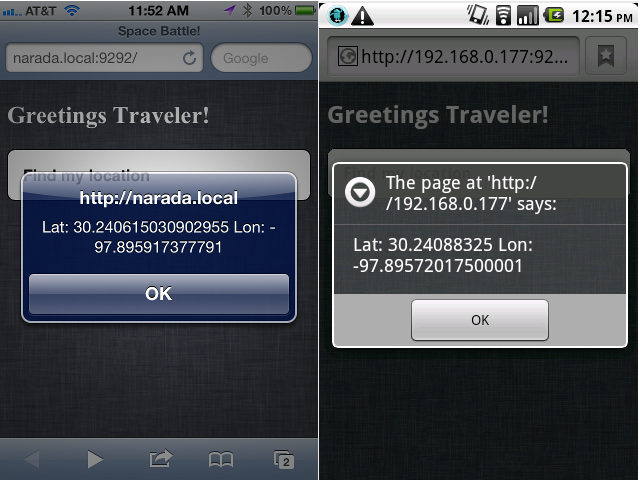
\includegraphics[scale=0.6]{1.png}
\caption{Geolocation API functioning in iOS and Android Browsers}
\label{geoloc}
\end{figure}

\subsection{iOS Customization}

Space Battle! is compatibile with most mobile web browsers, however there is 
some benefit to emulating a native app's look and feel. To facilitate this, 
iOS allows you to add HTML meta tags that enable
a web page bookmark to be saved to the device's ``home screen'' and allow 
custom HTML rendering behavior when using an iOS web browser. Space Battle! adds a splash
screen and creates a UI similar to what a native iOS app would look
like. When viewing the same HTML on an Android phone, it looks similar,
which allows for a solid cross platform interface. If a developer building 
an application with Marionette wants to have
access to more of the native iOS capabilities (e.g., mobile push) you can
package the HTML, CSS, and JavaScript together and create a native
Objective-C app that exposes the webpage through a
\texttt{UIWebView} class. An in-depth tutorial of
creating this support is available at \cite{mightios}.

\begin{figure}[h!]
\centering
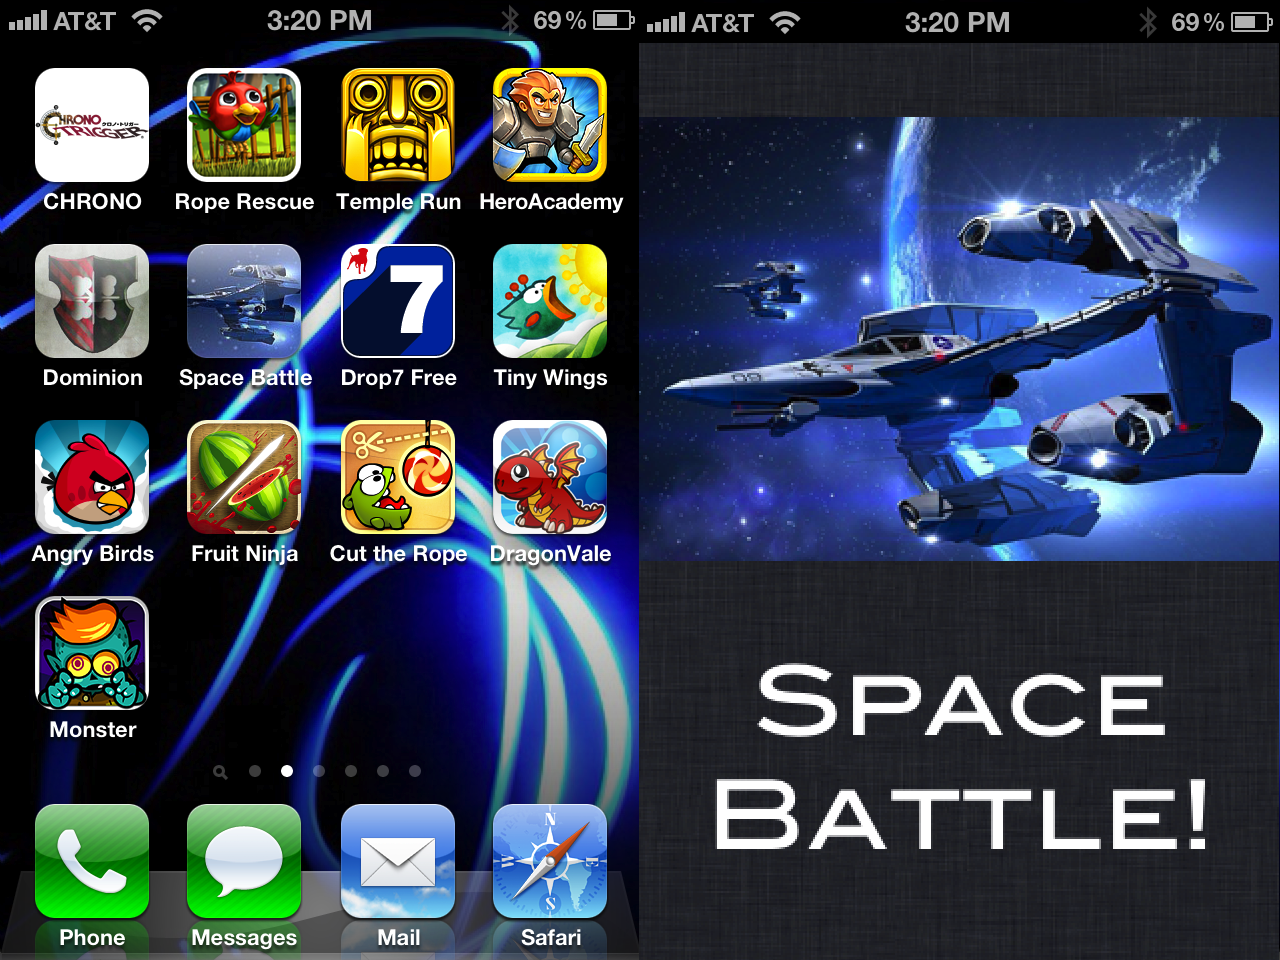
\includegraphics[scale=0.35]{2.png}
\caption{iOS Customized icon and splash screen}
\label{ioscustom}
\end{figure}

\chapter{Space Battle!}

\section{Basic Premise}

The basic premise of Space Battle! is to demonstrate a subset of basic
multiplayer online game mechanics within Marionette. Those mechanics
are: location, trade, and player vs. player combat. Starting a new game,
a player creates a new spaceship or if the player is returning, he can continue with a
spaceship that already exists. To board a spacecraft, the client
browser needs a location, which is provided by the Geolocation API. The
latitude and longitude queried are normalized into coordinates in a
reality overlay to where another player a mile or two away physically
would be relatively close in the game. Determining the exact
normalization factor would be an exercise best suited during gameplay
testing; for now the normalization factor is arbitrary.
The current implementation places starships within a 100x100 square grid
for ease of prototyping.

The reality overlay is organized into sectors (20 light-year (ly)
squares) and a given starship can perform long range sensor scans at a
radius of approximately 17 light-years. A starship has short range
sensors to about 500,000 kilometers (km). A given starship's weapon
range is 150,000 km. Firing on other starships causes damage to a starship's
components, eventually necessitating repair at in-game starbases run by
the game masters. Depending on a starship's coordinates relative to
other starships in the general vicinity, a player can perform a variety of
actions. This is a perfect use for the range query presented in
\cite{zio2011p2p}. The current implementation scales
down the vastness of space within a 100x100 2-D plane with 10x10
sectors; starships have a long range sensor scan radius of 8 and weapons
range is within a radius of 1.

The data storage mechanism relies on the use of WebSQL on the client web
browser instances. For purposes of replication, each client in a zone has
a copy of each event such that if a client drops the browser connection
the other nodes in the zone can potentially service the query. If a
zone's population approaches zero, it can instruct the remaining nodes to 
send a copy of the current events to neighboring zones. When a zone no longer 
has any occupants, it merges with an adjacent zone and queries resolve within 
the expanded zone. The current Marionette implementation does
not support this level of fault tolerance, but it could be added as the
framework develops.

\chapter{Overarching Design Considerations}

The communications backbone is centralized within Marionette because
mobile web browser connections are only open for as long as you are
viewing the page. On a mobile device, if a user context switches away from
the web browser to a different application, the WebSocket may have disconnected 
temporarily and may be unable to answer queries. Utilizing a 
centralized communications backbone
is the simplest way to maintain continuity between the web clients
within the scope of this work. No game specific data is stored on the
message broker. All pieces of the communications backbone (Sinatra,
Juggernaut, and Redis) are capable of scaling allowing room to grow 
should the need arise. With Juggernaut and Sinatra, one can spawn more 
instances behind a load balancer, and Redis supports replication.

\chapter{Implementation}

\begin{figure}[h!]
\centering
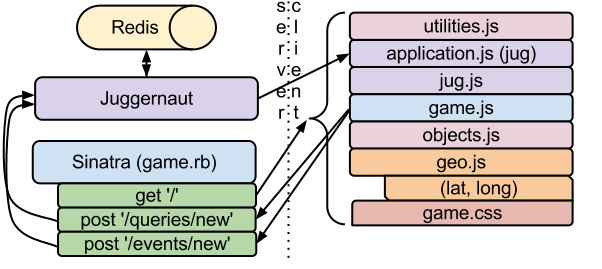
\includegraphics[scale=0.6]{3.png}
\caption{Marionette and Space Battle! files}
\label{files}
\end{figure}

\section{Marionette}

The Marionette framework consists of both server and client code. The
events and queries are sufficiently generalized to be utilized in a wide
variety of applications. Specialization can be accomplished via object-oriented 
inheritance or by injecting a serialized object inside an
event itself. Space Battle! opted to use simple type inheritance to
reduce the number of serialization and deserialization methods between
Ruby and Javascript. A client web browser pulls down all the javascript
by visiting the website's root with a GET request in HTML. Figure
\ref{files} shows the files that get pulled down by the
client browser on the right and all of the server files on the left. The
WebSQL database tables are created if they do not currently exist. The
server holds static counters for client\_id, event\_id, and query\_id.
Whenever the client browser makes a POST request intending for the
action to be published via Juggernaut, the server tacks on the unique id
and propagates the request to the applicable zones. The response to the
POST request contains the id that was assigned so the originating client
can update its records.

The jug.js file is responsible for instantiating the jug object defined
from application.js, which handles interaction with the Juggernaut
instance. The client browser can subscribe to any channel, and the
current implementation subscribes automatically to the channels shown in
Table \ref{jugzones}.

\ctable[pos = h, center, botcap, caption=Client channel subscriptions in Juggernaut, label=jugzones]{ll}
{% notes
}
{% rows
\FL
/global & global zone
\NN
/zones & zone management
\NN
/clients/:id & private channel for client
\NN
/zones/:id & channel for zone
\LL
}

Publishing to /global would send the content to all connected nodes. The
/zones channel is also global but used more often to propagate zone
updates. All nodes in a zone receive an event when a new zone is added, for example. 
When you subscribe to a channel, it executes a callback that the
Ruby server can listen to. The Ruby server can then assign a zone\_id
based on the current topology of nodes, which will then trigger the web
browser to subscribe to that zone. After the client has subscribed to
its zone, it then starts receiving queries that the client can begin
resolving.

\section{Space Battle!}

Space Battle! uses the Marionette framework to drive its gameplay
events. In the current implementation, only the scanning of other
starships is enabled via the use of the range query. Trade and combat
mechanics were not able to be implemented, but can be added in very
easily as they are built off the primitive query and event objects. Web
clients pilot a starship that has a location normalized into a 100x100
grid based on the device's geographic location. Once the ship is boarded,
it can then begin scanning for nearby ships via a range query. The range 
query in this case contains client's identification number, the device's 
present location, the radius of its sensor sweep, and the type of the object 
the starship is querying which is other starships. This can be expressed in 
shorthand as \texttt{RQ\{client\_id, (x,y), sensor\_distance, typeof(Starship)\}} 
The results
of that query will be a collection of other starships that matched and
their locations. If a starship is within a radius of one it is
considered to be within weapons range and can be fired upon. The
implementation is currently very simplistic, however it can be expanded
upon to increase gameplay and interaction value by adding more events
that can be queried via range query.

\section{Screenshots}

\begin{figure}[h!]
\centering
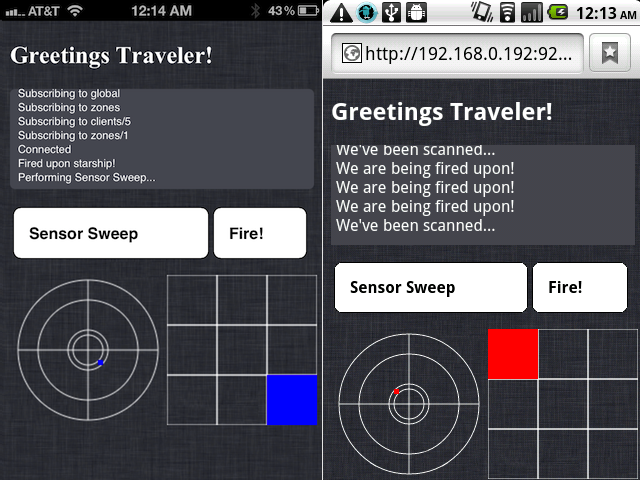
\includegraphics[scale=0.6]{4.png}
\caption{iOS and Android Screenshots}
\label{screenshot}
\end{figure}

An example game of Space Battle! is shown in Figure
\ref{screenshot}. The simplified game implementation
has a few UI buttons, a text console, and a couple of graphical gauges.
The gauge on the left shows the results of the sensor sweep, and the
gauge on the right shows if there are any ships within attack range.
Filled in squares on the right side indicate that there is a ship that
could be attacked and serves as a warning that a ship could attack
because they are within range themselves. The iOS customization
discussed previously has removed the address bar and the bottom button
bar shown in Figure \ref{geoloc} for a more native
feel. The Android screenshot shows that the game can run on Android web
browsers released two years ago as the device is running Android 2.1.

\chapter{Results}

\section{GitHub}

The implementation of Marionette and Space Battle! is published to
GitHub \cite{marionette}. The implementation will be
steadily enhanced over time as the framework matures as the concepts of
mobile multiplayer online gaming and grassroots information sharing are
explored. The code is licensed under a Creative Commons
Attribution-NonCommercial-ShareAlike (BY-NC-SA) license, which makes the
code accessible to those interested in studying and enhancing the
existing framework.

\section{Test Harness}

To test the interaction between multiple mobile clients, a test harness
was constructed that replicated mobile device connections as desktop
browser tabs. Using Watir bindings for Ruby, it is a fairly simple
matter to create multiple instances of Google Chrome, open multiple tabs
within each, and run a stress test that simulates user interaction.
Chrome is WebKit based so it represents a natural analog to a mobile web
browser. The only difference would be the processing power available to
the browser would likely be higher on a desktop than on a mobile device.
The goal of the test harness is to perform concurrent Sinatra/Juggernaut
accesses and see if the Marionette framework can handle some degree of
request concurrency. Unfortunately, the Chromium web driver was not
built to handle concurrent network accesses itself so the test randomly
ends after 1200 button presses. For each browser tab
the test harness provides a random location within the 100x100 grid and
provides a predefined client\_id. The current implementation only mashes
buttons to generate query and event traffic but could easily be modified
towards representing a simple artificial intelligence (AI) whose goal it
is to fire upon any starship within weapons range.

\chapter{Future Work}

There is a good deal of future work that builds on the progress from the
early implementation of Marionette and Space Battle!. Marionette could
be simplified to not build Ruby equivalent classes for the event and
query objects in Javascript since they are just getting passed to
Juggernaut. This was a remnant of an earlier idea that needs to be
cleaned up and would reduce the complexity of the serialization and
deserialization routines in Javascript. In the initial implementation,
all of the locations were relatively unchanged in the test harness. Some
work would need to be done towards deciding when to adjust the zone
allocations after a client has physically moved out of its originating
zone. The test harness can also be enhanced to move the starships around
the 100x100 grid to discover how to best tackle client migration as well
as outfit the simulated pilots with AI and tweak gameplay parameters
from there. Fault tolerance of the client nodes is also an area that
needs work based on the initial implementation.

\chapter{Conclusion}

This paper addressed the possibility of sharing of location-specific,
short-lived information between people using the web browser on their
mobile devices without requiring the installation of additional software
or proprietary plugins. To enable this level of communication between
mobile devices a new framework was presented, Marionette. It utilizes a
pub-sub service in conjunction with events distributed amongst the
client devices that could be queried by means of a range query. This
technique would allow the creation of grassroots information sharing
relative to the user's surroundings. This paper also presented a mobile
multiplayer online game called Space Battle!, which utilizes Marionette
as a means of communicating game events to other mobile devices. Several
multiplayer online game mechanics work well with the event and query
model that Marionette provides. Explorations with respect to the
Marionette framework need to be further explored in the future, however
the Space Battle! game serves as an adequate basic implementation and
demonstration of the ideas presented herein.

%%%%%%%%%%%%%%%%%%%%%%%%%%%%%%%%%%%%%%%%%%%%%%%%%%%%%%%%%%%%%%%%%%%%%%
% Appendix/Appendices                                                %
%%%%%%%%%%%%%%%%%%%%%%%%%%%%%%%%%%%%%%%%%%%%%%%%%%%%%%%%%%%%%%%%%%%%%%
%
% If you have only one appendix, use the command \appendix instead
% of \appendices.
%
%\appendices
%\index{Appendices@\emph{Appendices}}%

%\include{chapter-appendix1}

%\include{chapter-appendix2}

%\include{chapter-appendix3}


%%%%%%%%%%%%%%%%%%%%%%%%%%%%%%%%%%%%%%%%%%%%%%%%%%%%%%%%%%%%%%%%%%%%%%
% Generate the bibliography.					     %
%%%%%%%%%%%%%%%%%%%%%%%%%%%%%%%%%%%%%%%%%%%%%%%%%%%%%%%%%%%%%%%%%%%%%%
%								     %
% NOTE: For master's theses and reports, NOTHING is permitted to     %
%	come between the bibliography and the vita. The command      %
%	to generate the index (if used) MUST be moved to before      %
%	this section.						     %
%								     %
\nocite{*}      % This command causes all items in the 		     %
                % bibliographic database to be added to 	     %
                % the bibliography, even if they are not 	     %
                % explicitly cited in the text. 		     %
		%						     %
\bibliographystyle{plain}  % Here the bibliography 		     %
\bibliography{masters_report}        % is inserted.			     %
\index{Bibliography@\emph{Bibliography}}%			     %
%%%%%%%%%%%%%%%%%%%%%%%%%%%%%%%%%%%%%%%%%%%%%%%%%%%%%%%%%%%%%%%%%%%%%%


%%%%%%%%%%%%%%%%%%%%%%%%%%%%%%%%%%%%%%%%%%%%%%%%%%%%%%%%%%%%%%%%%%%%%%
% Generate the index.						     %
%%%%%%%%%%%%%%%%%%%%%%%%%%%%%%%%%%%%%%%%%%%%%%%%%%%%%%%%%%%%%%%%%%%%%%
%								     %
% NOTE: For master's theses and reports, NOTHING is permitted to     %
%	come between the bibliography and the vita. This section     %
%	to generate the index (if used) MUST be moved to before      %
%	the bibliography section.				     %
%								     %
%\printindex%    % Include the index here. Comment out this line      %
%		% with a percent sign if you do not want an index.   %
%%%%%%%%%%%%%%%%%%%%%%%%%%%%%%%%%%%%%%%%%%%%%%%%%%%%%%%%%%%%%%%%%%%%%%


%%%%%%%%%%%%%%%%%%%%%%%%%%%%%%%%%%%%%%%%%%%%%%%%%%%%%%%%%%%%%%%%%%%%%%
% Vita page.							     %
%%%%%%%%%%%%%%%%%%%%%%%%%%%%%%%%%%%%%%%%%%%%%%%%%%%%%%%%%%%%%%%%%%%%%%

\begin{vita}
Benjamin Mark Cochran was born in northern Indiana in 1982. He graduated
with honors from Penn High School in Mishawaka, IN in 2001 and was a
member of the FIRST Robotics team his senior year. During undergraduate
studies he was a member of Theta Tau, the oldest, largest and foremost
Fraternity for Engineers. He received his Bachelor of Science degree in
Computer Engineering from Purdue University in 2005. Shortly after
graduation in early 2006 he accepted a position at Advanced Micro
Devices (AMD) in Austin, TX as a Product Development Engineer focusing
on DDR and HyperTransport I/O interfaces and test automation. In early
2010, he began graduate studies at the University of Texas at Austin,
pursuing a Master of Science in Engineering degree. He is passionate
about emerging web technologies, mobile computing, test automation, and
software engineering best practices. In his free time he enjoys fine
beers, video games, mountain biking, and watching movies at the Alamo
Drafthouse.
\end{vita}

\end{document}
